\documentclass[12 pt]{beamer}
\usetheme[
  bullet=circle,		% Other option: square
  bigpagenumber,		% circled page number on lower right
  topline=true,			% colored bar at the top of the frame 
  shadow=false,			% Shading for beamer blocks
  watermark=BG_lower,	% png file for the watermark
]{Flip}


\newcommand{\titleimage}{title}			% Custom title 
\newcommand{\tanedo}{tanedolight}		% Custom author name
\newcommand{\CMSSMDM}{CMSSMDMlight.png}	% light background plot


%%%%%%%%%%
% FONTS %
%%%%%%%%%%

\usepackage[T1]{fontenc}
%\usepackage{lmodern}		
%\usepackage{sfmath}		% Sans Serif Math, off by default

%% Protects fonts from Beamer screwing with them
%% http://tex.stackexchange.com/questions/10488/force-computer-modern-in-math-mode
\usefonttheme{professionalfonts}


\usepackage[no-math]{fontspec}		

%\defaultfontfeatures{Mapping=tex-text}	% This seems to be important for mapping glyphs properly

\usepackage{amsmath}
%\usepackage{amsfonts}
%\usepackage{amssymb}
\usepackage{mathspec}
\usepackage{graphicx}
%\usepackage{mathrsfs} 			% For Weinberg-esque letters
\usepackage{cancel}				% For "SUSY-breaking" symbol
\usepackage{slashed}            % for slashed characters in math mode
%\usepackage{bbm}                % for \mathbbm{1} (unit matrix)
\usepackage{amsthm}				% For theorem environment
\usepackage{multirow}			% For multi row cells in table
\usepackage{arydshln} 			% For dashed lines in arrays and tables
\usepackage{tikzfeynman}		% For Feynman diagrams
% \usepackage{subfig}           % for sub figures
% \usepackage{young}			% For Young Tableaux
% \usepackage{xspace}			% For spacing after commands
% \usepackage{wrapfig}			% for Text wrap around figures
% \usepackage{framed}

\usepackage{setspace}

\setsansfont{calibri}[ 
Extension = .ttf,
UprightFont = *,
BoldFont = *b,
ItalicFont = *i,
Scale = 1
]

\setmathfont(Digits,Latin,Greek){SitkaI.ttc}

\graphicspath{{images/}}	% Put all images in this directory. Avoids clutter.


\usetikzlibrary{backgrounds}
\usetikzlibrary{mindmap,trees}	% For mind map
\usetikzlibrary{arrows,positioning,calc}
\usetikzlibrary{shapes}
% http://www.texample.net/tikz/examples/computer-science-mindmap/


% SOME COMMANDS THAT I FIND HANDY
% \renewcommand{\tilde}{\widetilde} % dinky tildes look silly, dosn't work with fontspec
\newcommand{\comment}[1]{\textcolor{comment}{\footnotesize{#1}\normalsize}} % comment mild
\newcommand{\Comment}[1]{\textcolor{Comment}{\footnotesize{#1}\normalsize}} % comment bold
\newcommand{\COMMENT}[1]{\textcolor{COMMENT}{\footnotesize{#1}\normalsize}} % comment crazy bold
\newcommand{\Alert}[1]{\textcolor{Alert}{#1}} % louder alert
\newcommand{\ALERT}[1]{\textcolor{ALERT}{#1}} % loudest alert
%% "\alert" is already a beamer pre-defined



\author{}
\title{Informatikai Rendszerek Biztonságtechnikája}
\institute{}
\date{}



\begin{document}

%% To use external nodes; http://www.texample.net/tikz/examples/beamer-arrows/
\tikzstyle{every picture}+=[remember picture]

{
  \setbeamertemplate{sidebar right}{\llap{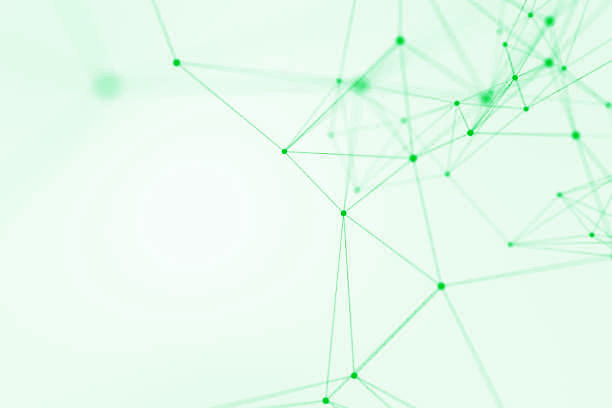
\includegraphics[width=\paperwidth,height=\paperheight]{backgnd}}}

  \begin{frame}[c]
    \begin{center}
      % \includegraphics[width=7cm]{WarpedPenguinsReturn}

      \Large
      \textbf{Információs rendszerek}

      \textbf{biztonságtechnikája}

      \qquad

      Kriptográfia

      Kriptográfiai hash algoritmusok

      \qquad

      \textit{Vakulya Gergely}

    \end{center}
  \end{frame}
}

  %------------------------------------------------

\begin{frame}{Hash mint adatstruktóra}
    \begin{itemize}
      \item{A hash adatszerkezet lényege, hogy elemeket egy $k$ db rekeszt tartalmazó tárolóban elhelyezzünk úgy, hogy azokhoz azonnal (keresés nélkül) hozzáférjünk.}
      \item{Ehhez minden elem értéke alapján egy bélyeget (hash-t) generáljunk. Ez adja a rekesz sorszámát.}
      \item{Célok:}
        \begin{itemize}
          \item{A tárolni kívánt elemszámhoz minél kisebb ($k$ szmú) rekesz kelljen.}
          \item{Ne kerüljön egy rekeszbe egynél több elem (kerüljük el a \textbf{hash ütközést}).}
        \end{itemize}
      \item{Számos módszer született (például osztásos, szorzásos, Fibonacci hasítás)}
      \item{Az adott célra használhatunk saját algoritmust is.}
      \item{A hash függvény $k$ rekeszhez egy $\lceil log_{2}(k) \rceil$ bites számot rendel.}
      \item{Akár a tárolandó adat első byte-ja is használható hasz-ként.}
    \end{itemize}
\end{frame}

\begin{frame}{A kriptográfiai hash algoritmusok}
  \begin{itemize}
    \item{A kriptográfiai hash algoritmus is egy azonosítót (hash-t, \textbf{üzenet pecsétet}) rendel a bejövő adathoz.}
    \item{Itt is fontos szempont, hogy \textbf{ne legyen hash ütközés}.}
    \item{A hash-nek \textbf{egyirányúnak} kell lennie, azaz belőle ne lehessen következtetni az bemenő adatra, vagy annak egy részére.}
    \item{Nem cél, hogy egy $b$ bites hash esetén a virtuálisan létrejövő $k = 2^b$ db rekeszt minél jobban kihasználjuk.}
    \item{A gyakorlatban előforduló felhasználási módok:}
      \begin{itemize}
        \item{Üzenetek (fájlok) \textbf{integritásának} ellenőrzése.}
        \item{A \textbf{digitális aláírás} egyik fontos eszköze.}
        \item{\textbf{Jelszavak} tárolása}
      \end{itemize}
    \item{Fontosabb kriptográfiai hash algoritmusok: MD-5, SHA-1, SHA-2. Láthatáron az SHA-3.}
  \end{itemize}
\end{frame}

\begin{frame}{Az MD-5 hash algoritmus}
  \begin{itemize}
    \item{MD-5: Message Digest 5.}
    \item{Ronald Rivest, 1992 (ő az a Rivest, aki az RSA-ból az R betű).}
    \item{128 bites üzenet pecsétet állít elő.}
    \item{Sokáig ez volt de facto standard, de ma már elavultnak számít.}
    \item{A 2004-es kiadású Számítógép hálózatok könyvben még biztonságosnak említik.}
    \item{Azóta már gyorsan generálhatóak szándékosan ütköző file-ok.}
    \item{\href{https://github.com/corkami/collisions}{https://github.com/corkami/collisions}}
    \item{Linux parancs: \texttt{md5sum}}
  \end{itemize}
\end{frame}

\begin{frame}{Az SHA-1 hash algoritmus}
  \begin{itemize}
    \item{Secure Hash Algorithm 1.}
    \item{1995-ben publikálták.}
    \item{Az AES-hez hasonlóan ez is amerikai kormányzati megbízásból készült.}
    \item{Belső felépítése hasonló az MD-5-éhez, de 160 bites üzenet pecsétet állít elő.}
    \item{Biztonságosabb, mint az MD-5, de megfelelő anyagi ráfordítással sebezhető.}
    \item{Gyengesége miatt egyre kevésbé támogatott.}
    \item{Linux parancs: \texttt{sha1sum}}
  \end{itemize}
\end{frame}

\begin{frame}{Az SHA-2 hash algoritmuscsalád}
  \begin{itemize}
    \item{Secure Hash Algorithm 2.}
    \item{Az NSA publikálta 2001-ben.}
    \item{Több különböző méretű hash-t is elő tud állítani}
      \begin{itemize}
        \item{256 és 512 bites fő működési módok (SHA-256 és SHA-512).}
        \item{A 256 bites kimenet 224 bitre csonkolható kis mértékű belső változtatással (SHA-224).}
        \item{Az 512 bites kimenet 224, 256 és 384 bitre csonkolható kis mértékű belső változtatással (SHA-512/224, SHA-512/256 és SHA-384)}
      \end{itemize}
    \item{Linux parancsok: \texttt{sha224sum}, \texttt{sha256sum}, \texttt{sha384sum}, \texttt{sha512sum}, \texttt{shasum}}
  \end{itemize}
\end{frame}

\begin{frame}{Kriptoanalízis}
  \begin{block}{A lehetséges támadások típusai}
    \begin{itemize}
      \item{Egy adott hash-hez tartozó tartalom (fájl) előállítása: Közel lehetetlen.}
      \item{Egy adott fájlhoz tartozóval megegyező hash-sel rendelkező másik fájl előállítása: Lényegében azonos az előzővel, így közel lehetetlen.}
      \item{Két kölönböző (tetszőleges) fájl előállítása, amik ugyanazt a hash-t adják: lehetséges (születésnap támadás, elég lassú)}
      \item{Két megadott fájlkezdethez olyan kiegészítések előállítása, hogy a kiegészített fájlok ugyanazt a hash-t adják: lehetséges (prefix/append támadások, néhány napos számítási idő)}
      \item{Két különböző, de megadott megjelenést adó fájl előállítása, amik ugyanazt a hash-t adják: lehetséges (másodperces nagyságrendű számítási idő)}
    \end{itemize}
  \end{block}
\end{frame}

\begin{frame}{A születésnap támadás (birthday attack)}
  \begin{block}{Születésnap paradoxon}
    \begin{itemize}
      \item{Meglepően kis létszámú (23 fős) csoportban már legalább 50\% a valószínűsége annak, hogy két ember ugyanazon a napon ünnepli a születésnapját.}
      \item{A párok száma: $\frac{23 \cdot 22}{2} = 253$}
      \item{A lehetséges napok száma: 365.}
      \item{Minden esetben $\frac{1}{365}$ a valószínűsége annak, hogy azonos napon születtek.}
    \end{itemize}
  \end{block}

  \begin{block}{Következmény a hash-ekre nézve}
    \begin{itemize}
      \item{Egy $n$ bites hash algoritmust alapul véve $2^{\frac{n}{2}+1}$ darab fájl esetén valószínűleg lesz a halmazban ütközés.}
      \item{Hasonlóan egy $2^\frac{k}{2}$ elemszámú és egy másik, szintén $2^\frac{k}{2}$ elemszámú halmaz elemei között valószínűleg találunk azonos hash-t adó párt.}
    \end{itemize}
  \end{block}
\end{frame}

\begin{frame}{A születésnap támadás kihasználása}
  \begin{itemize}
    \item{Tegyük fel, hogy egy üzleti partnerrel szeretnénk szerződést kötni úgy, hogy mi lényegesen jobban járjunk, mint partnerünk.}
    \item{Elkészítünk egy ,,fair'' szerződésből $2^\frac{2}{2}$ kinézetre azonos, de bit szinten különböző példányt, illetve egy ,,kizsákmányoló'' verzióból is ugyanennyit.}
    \item{Keresünk egy olyan párt, a ,,fair'' és a ,,kizsákmányoló'' verzió hash-e azonos.}
    \item{Elküldjük a ,,fair'' verziót, valamint annak hash-ét partnerünknek.}
    \item{Elküldjük a ,,kizsákmányoló'' verziót annak (megegyező) hash-ével az ügyvédünknek.}
    \item{Ennek jelentőségét majd a digitális aláírásoknál fogjuk megérteni.}
  \end{itemize}
\end{frame}

\begin{frame}{Jelszavak tárolása hash formájában}
  \begin{itemize}
    \item{A hash algoritmusok jelszavak kezelésére is alkalmasak}
    \item{A különböző rendszerek (webalkalmazások, operációs rendszerek) nem magát a jelszót tárolják, hanem annak hash-ét.}
    \item{Valójában nem magát a hash-t tárolják, hanem a jelszót először kiegészítik egy véletlenszerű szöveggel és ennek a hash-ét tárolják (sózott jelszó).}
    \item{Sőt leggyakrabban több körös sózás -- hash-elés kombinációt alkalmaznak (PBKDF2, Password Based Key Derivation Function 2)}
  \end{itemize}
\end{frame}

\begin{frame}{Jelszótárolás kriptoanalízise, szivárványtábla}
  \begin{itemize}
    \item{A gyakori / egyszerű jelszavak hash-ei előre legenerálhatóak (szivárványtábla, rainbow table)}
    \item{A rendszerünkből kiszivárgott hash-eket gyorsan rá lehet próbálni a szivárványtáblában szereplőkre.}
    \item{Sózott jelszó esetén minden kipróbált jelszóhoz generálni kell a hash-t (lassabb).}
    \item{Többszáz körös sózás -- hash-elés (PBKDF2) esetén többmillió potenciális jelszó hash-ének generálása igen lassúvá válik.}
  \end{itemize}
\end{frame}

%Public-Key Cryptography Standards (PKCS)

\end{document}
